\subsection{Physical processes}

The general physical properties of the media (such as density, atomic weights, atomic numbers etc.) are used by {\geant}4 to simulate interactions of the particles with detector materials (e.g. Bremsstrahlung, ionization, production of secondary particles). If a material has, in addition, Cherenkov properties, then a particle can emit Cherenkov photons inside this material. The expectation value of the number of Cherenkov photons emitted per unit of trajectory $dN/dx$ is calculated according to the Frank-Tamm equation. During the propagation process of a charged particle inside the material with Cherenkov properties the number of photons produced within each step is generated according to a Poisson distribution with the mean of $\langle n \rangle = L_{step} \cdot dN/dx$. After the photons are produced they are propagated individually through the detector materials. The particles are transported inside the detector volume in an iterative process to discrete positions with a certain step size. At each of these positions a detector-specific routine is called by the {\geant}4 in order to process the simulated information inside its sensitive volumes. There, the current particle state (e.g. momentum, type, and mother-daughter relation) and the relevant processes during the current step (e.g. reflection, refraction) are available.

A high momentum charged particle produces at the order of $1000$ photons per cm of fused silica in the wavelength range $(300-700)$ nm. Only $30-60$ of them are expected to be detected. Typical Cherenkov photon energies are in the range of few eV. For proper estimation of the detector performance it is very important to predict realistic photon yields. Common reasons why a Cherenkov photon is not detected are the following:

\begin{itemize}
\item The material, where the Cherenkov photons is produced or currently propagating, might be non-transparent for the given wavelength -- the photon stops (after some distance, depending on the defined absorption length as a function of wavelength for the given medium);
\item The photon does not satisfy the total internal reflection condition at the border between the radiator and the surrounding air or nitrogen (and other interfaces) -- the photon leaves the radiator (or, more generally, the optical system of the detector) and is lost;
\item Some photons are reflected back on an interface between media with different refraction indices -- the photon is trapped inside some volume (or group of volumes);
\item The photon is not detected because of the photon detection efficiency of the sensors (the quantum efficiency for H12700 MaPMTs is shown in Fig.~\ref{pic:qe}) or the transport efficiency in the radiator (described below)  -- the photon reaches the photosensor, but is not detected.
\end{itemize}

The physical processes in the materials are simulated by {\geant}4 based on the Cherenkov properties. The processes of total internal reflection, chromatic dispersion, transmission, and absorption of Cherenkov photons inside the optical elements of the \gluex DIRC are treated by {\geant}4, too.

A fraction of Cherenkov photons emitted by a charged particle, gets trapped inside the radiator due to the total internal reflection effect. They need to be transported from the origin to the readout end of the radiator bar. Cherenkov photons usually undergo about several hundreds internal reflections inside a long \babar DIRC bars on the way towards the readout end. The sides of the radiator in the reality are not perfect, and surface roughness causes a photon to get scattered in a random direction or escape from the radiator. In the simulation the radiator sides are perfectly polished leading to the fraction of transported photons to be $100\%$. In general, there are two ways to implement realistic transport efficiency into the simulation:

\begin{itemize}
\item The functionality of {\geant}4 (unlike Geant3) allows definition of an ``optical surface'' between two media with custom properties such as reflectivity and roughness. Then at each reflection off the radiator side, {\geant}4 decides according to the surface properties, to stop the photon or continue its transportation. It might be not straightforward to implement experimental results of the surface roughness measurements and make sure the simulation agrees with the measured data.
\item Transport efficiency can be calculated at the production stage for each photon based on the reflection probability and the total number of reflections off the sides. This speeds up the simulation. Also, the photon transport efficiency, which includes effects from the surface roughness and sub-surface damage, was experimentally measured for the \babar DIRC bard for several wavelength~\cite{roughness} and is, therefore, easy to implement.
\end{itemize}

We decided to follow the second method and apply the transport efficiency at the production stage as the following. The probability $P$ for a single reflection on the radiator side depends on the photon wavelength $\lambda$, incident angle of the photon $\alpha$, refraction index $n$, and the surface roughness $r$. According to scalar theory~\cite{scalar}:

\begin{equation}
P \approx  1 - \left( \frac{4\pi \cdot r \cdot \cos(\alpha) \cdot n(\lambda)}{\lambda} \right)^{2}, r \ll \lambda
\end{equation}

\begin{figure}[!h]
\centering
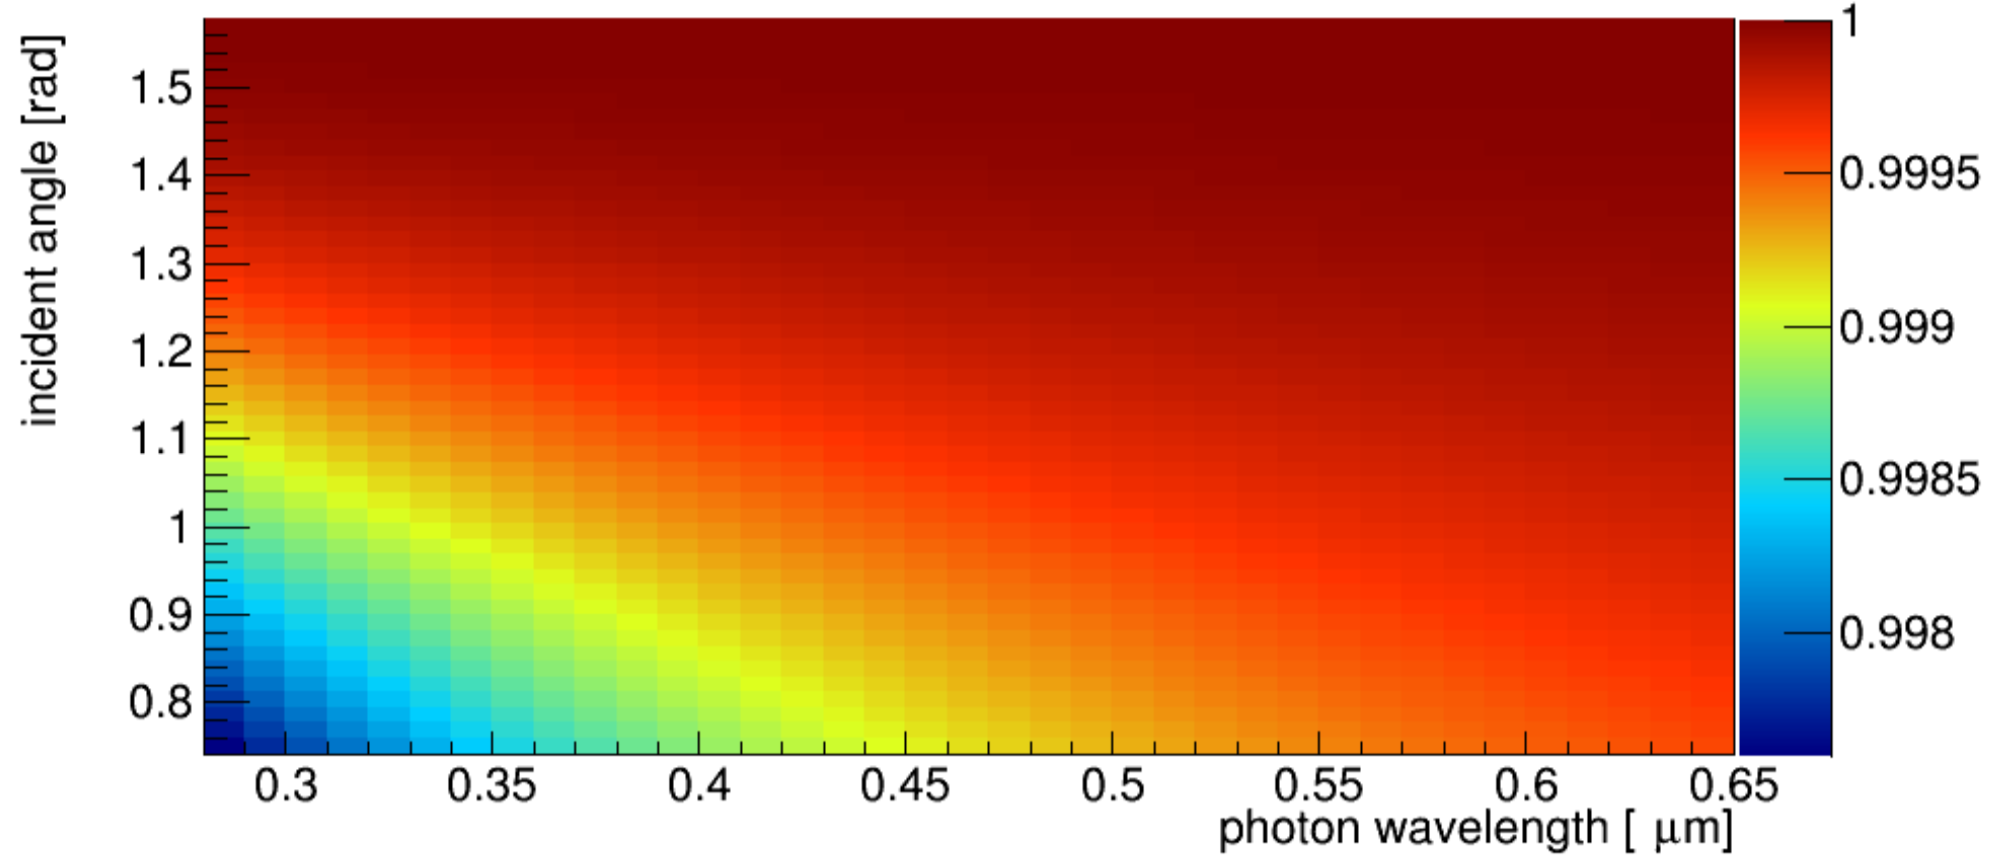
\includegraphics[width=0.8\textwidth]{pics/psurf.png}
\caption{\label{pic:sur}
Reflection coefficient $P$ as a function of the wavelength and incident angle of the Cherenkov photon.
}
\end{figure}

$P(\lambda,\alpha)$ is illustrated in Fig.~\ref{pic:sur}. The probability to survive the transpotation through the radiator can be calculated as $P_{total} = P^{N}$. Here $P_{total}$ is the transport efficiency for a given photon, and $N$ is the total number of reflections inside the radiator. We used experimental data of the transport efficiency, which agrees with the scalar theory for roughness value of $r \approx 5 A$~\cite{roughness}. Fig.~\ref{pic:tra} illustrates the impact of the transport efficiency on the photon yield for tracks hitting the bar (bar number 24 or 0 in Fig.~\ref{pic:dirc2}) closest to the beamline in different points along the $x$ axis. The effect is larger in the middle and decreases towards the ends of the bar. This correlates with the orientation of the Cherenkov cone inside the radiator: when a charged particle hits the middle of the bar, the Cherenkov cone is oriented perpendicularly to it, and photons have more reflections on the radiator sides than for the case when the charged particle traverses the bar at a more shallow angle.

\begin{figure}[!h]
\centering
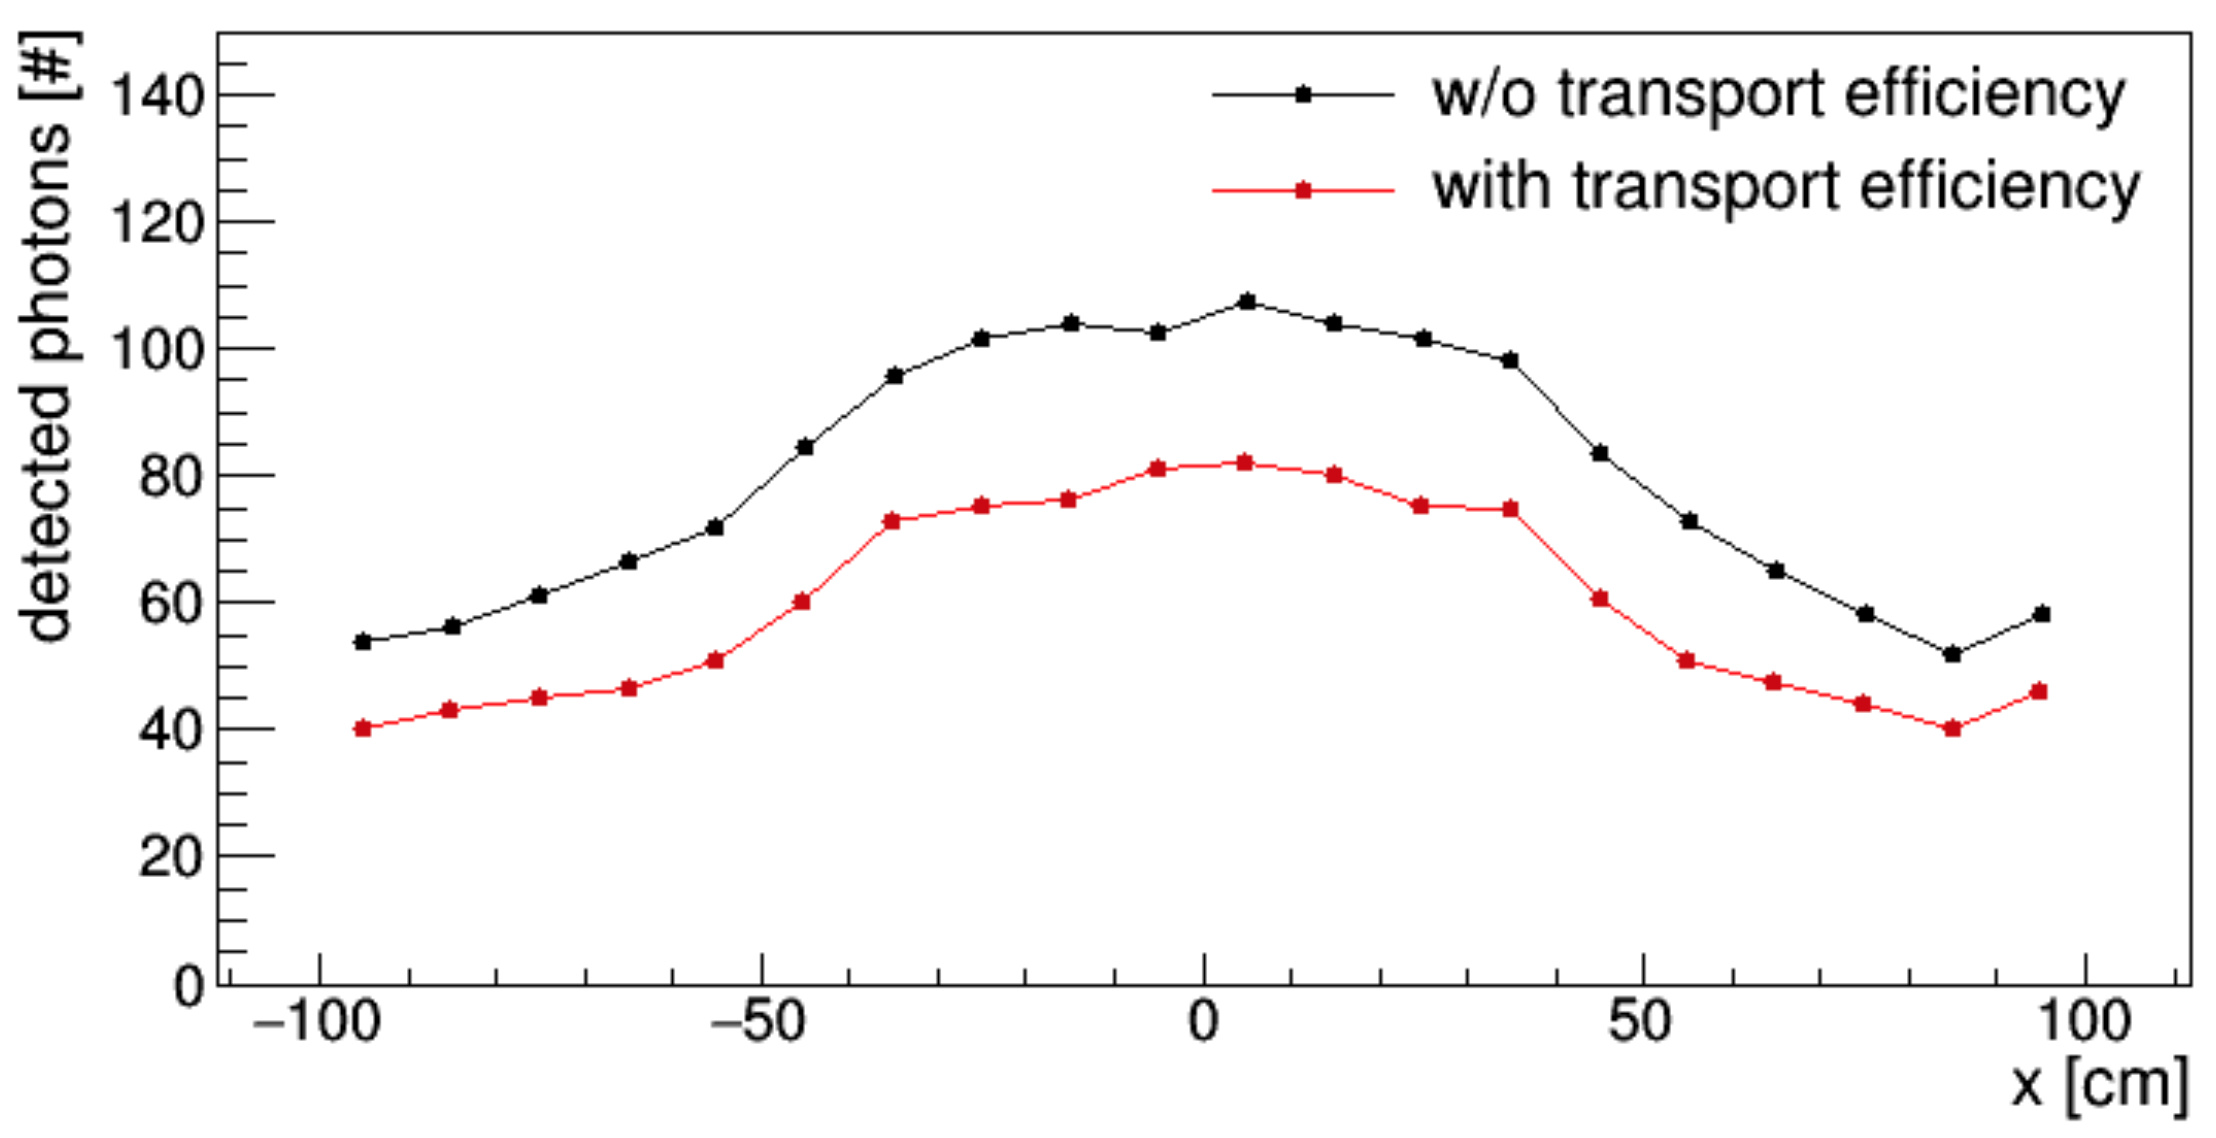
\includegraphics[width=0.8\textwidth]{pics/transport.png}
\caption{\label{pic:tra}
Impact of the transport efficiency on the photon yield. The study is based on $100k$ of $h'(2600)$ events. The photon yield is shown for the bar closest to the beamline (bar number 24 or 0 in Fig.~\ref{pic:dirc2}).
}
\end{figure}

The photon sensors are implemented in the simulation as a set of functional layers (see Fig.~\ref{pic:struct}). Propagation of Cherenkov photons through them is handled by {\geant}4. The detection efficiency, represented by the quantum efficiency (QE) of the photosensors (see Fig.~\ref{pic:qe}), is applied at the production stage to avoid tracing photons which are not going to be detected. Currently, the typical QE, same for all the sensors, is implemented. \textcolor{red}{QE values from the JLab scan? How uniform is the QE?} 

\begin{figure}[tb]
\centering
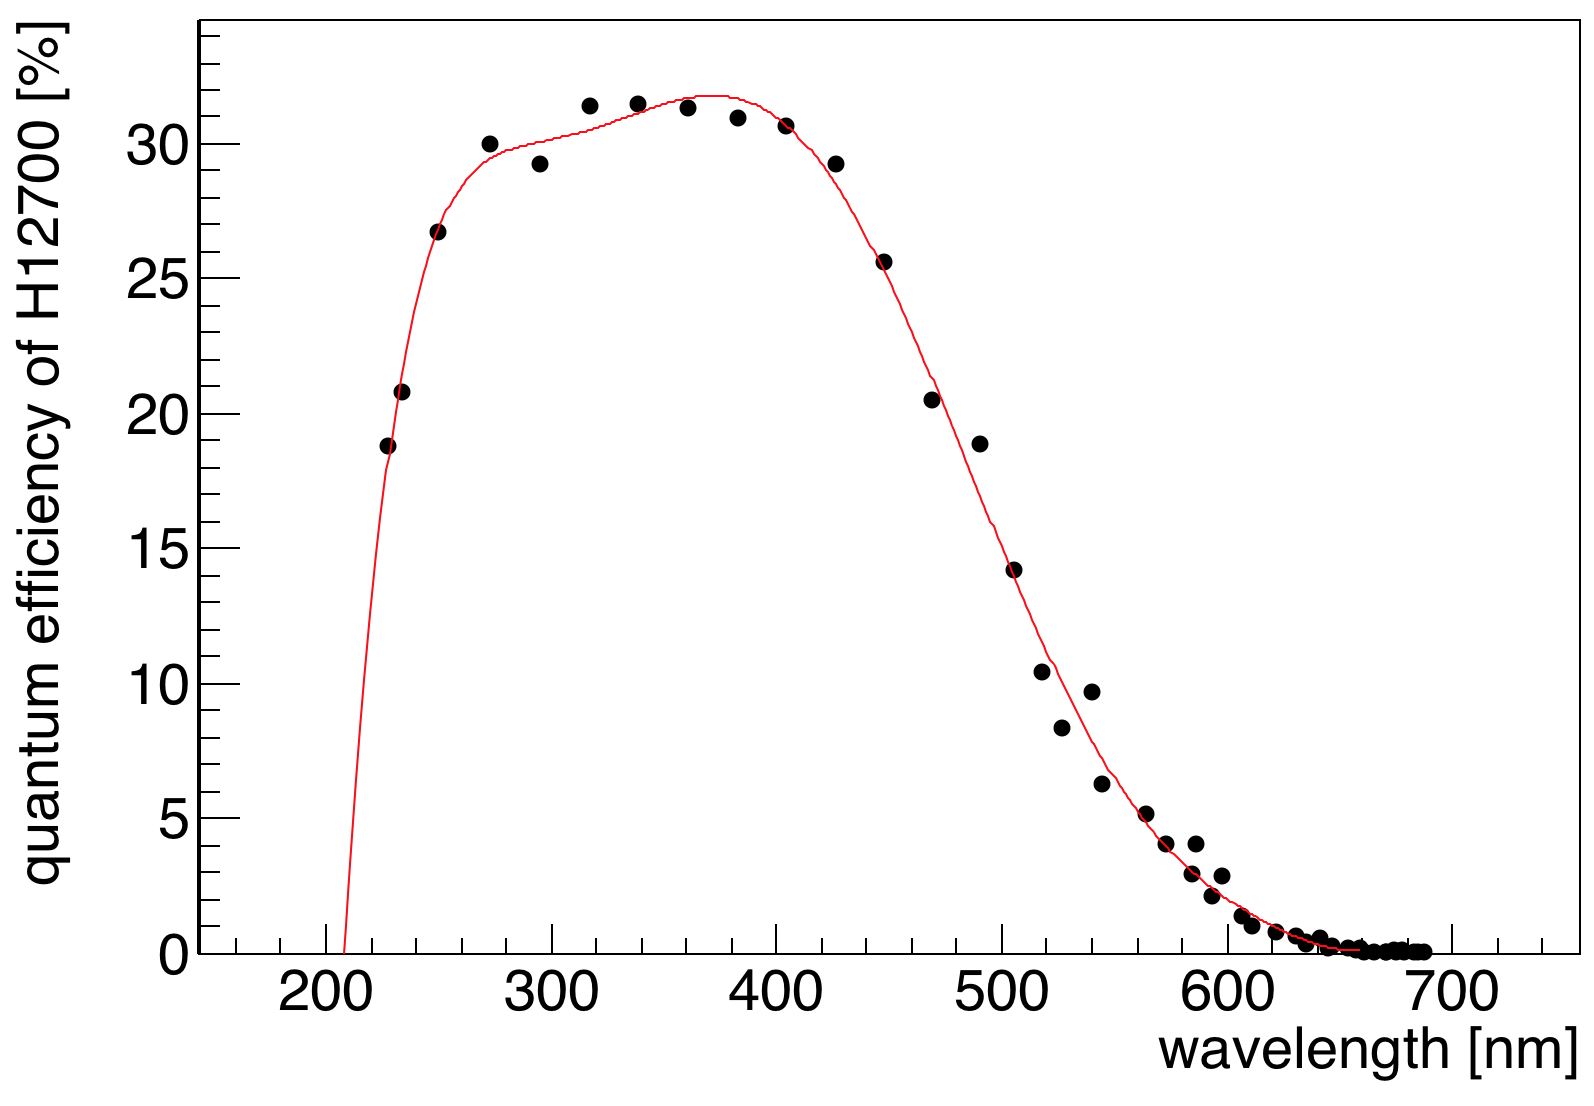
\includegraphics[width=0.5\textwidth]{pics/qe.png}
\caption{\label{pic:qe}
Quantum efficiency of photosensors Hamamatsu H12700. The red line shows a fit to the data points, extracted from the data sheet.
}
\end{figure}

The deterioration effects caused by imperfections of the physical shape of the radiators are not taken into account. The radiator bars in the detector simulation are perfect parallelepipeds, unlike in reality. Therefore, systematic smearing of the photon direction at every reflection inside the real radiator, which introduces an additional error to the reconstructed photon direction and therefore, to the obtained Cherenkov angle, is not (yet) taken into account.
